\documentclass[12pt, a4paper]{article}

% Packages
\usepackage[utf8]{inputenc}
\usepackage[T1]{fontenc}
\usepackage{geometry}
\usepackage{titlesec}
\usepackage{enumitem}
\usepackage{booktabs}
\usepackage{longtable}
\usepackage{array}
\usepackage{hyperref}
\usepackage{graphicx}
\usepackage{amsmath, amssymb}
\usepackage{listings}
\usepackage{xcolor}
\usepackage{fancyhdr}
\usepackage{caption}
\usepackage{subcaption}
\usepackage{tabularx}
\usepackage{float}
\usepackage{tikz}
\usetikzlibrary{shapes, arrows.meta, positioning, calc, fit}

\geometry{margin=1in}

\hypersetup{
    colorlinks=true,
    linkcolor=blue!70!black,
    urlcolor=blue!70!black,
    citecolor=blue!70!black
}

\lstset{
    basicstyle=\ttfamily\small,
    backgroundcolor=\color{gray!8},
    frame=single,
    breaklines=true,
    keywordstyle=\color{blue!80!black},
    commentstyle=\color{green!50!black},
    stringstyle=\color{red!70!black},
    numbers=left,
    numberstyle=\tiny\color{gray},
    numbersep=8pt,
    showstringspaces=false,
    tabsize=4
}

\pagestyle{fancy}
\fancyhf{}
\fancyhead[L]{\small Smart City Traffic Management}
\fancyhead[R]{\small Technical Specifications v2.0}
\fancyfoot[C]{\thepage}
\renewcommand{\headrulewidth}{0.4pt}

% Custom colors
\definecolor{headerblue}{RGB}{41, 65, 122}
\definecolor{lightgray}{RGB}{245, 245, 245}
\definecolor{accentgreen}{RGB}{34, 139, 34}

% =============================================================================
% TITLE PAGE
% =============================================================================
\begin{document}

\begin{titlepage}
\begin{center}

\vspace*{1.5cm}

{\Huge \textbf{Smart City Traffic Management System}}

\vspace{0.8cm}

{\LARGE Technical Specifications Document}

\vspace{0.5cm}

{\large Version 2.0}

\vspace{2cm}

\begin{tabular}{ll}
    \textbf{Project:} & Smart City Traffic Management \\
    \textbf{Course:} & RDMU --- Research Design and Methods \\
    \textbf{Program:} & MAIB --- Masters in AI with Business \\
    \textbf{Term:} & Term 2, 2025--2026 \\
    \textbf{Group:} & Group 2 \\
\end{tabular}

\vspace{2cm}

\textbf{Team Members}

\vspace{0.3cm}

\begin{tabular}{l}
    Kartik Joshi \\
    Anurag Deverakonda \\
    Nandana Santosh \\
    Weiqi Liu \\
    Advait Dalvi \\
    Gautam Barai \\
\end{tabular}

\vfill

\textbf{Date:} April 1, 2026

\end{center}
\end{titlepage}

% =============================================================================
% DOCUMENT CONTROL
% =============================================================================
\newpage

\section*{Document Control}

\subsection*{Revision History}

\begin{tabularx}{\textwidth}{|c|c|l|X|}
    \hline
    \textbf{Version} & \textbf{Date} & \textbf{Author(s)} & \textbf{Description} \\
    \hline
    1.0 & Mar 15, 2026 & Kartik Joshi, Anurag D. & Initial draft: architecture, state/action space, RL agents \\
    \hline
    1.1 & Mar 22, 2026 & Nandana S., Weiqi Liu & Added MCDM specification, synthetic data schema \\
    \hline
    1.2 & Mar 28, 2026 & Advait Dalvi, Gautam B. & Dashboard specification, deployment architecture \\
    \hline
    2.0 & Apr 1, 2026 & All members & Final version: neighbor awareness, XAI, chaos mode, economic analysis \\
    \hline
\end{tabularx}

\subsection*{Distribution List}

\begin{tabular}{ll}
    \toprule
    \textbf{Name} & \textbf{Role} \\
    \midrule
    Course Instructor & Reviewer / Evaluator \\
    Group 2 Members & Authors / Developers \\
    \bottomrule
\end{tabular}

\subsection*{Document Approval}

\begin{tabular}{lll}
    \toprule
    \textbf{Role} & \textbf{Name} & \textbf{Date} \\
    \midrule
    Project Lead & Kartik Joshi & Apr 1, 2026 \\
    Technical Lead & Anurag Deverakonda & Apr 1, 2026 \\
    \bottomrule
\end{tabular}

\newpage
\tableofcontents
\newpage
\listoftables
\listoffigures
\newpage

% =============================================================================
% 1. INTRODUCTION
% =============================================================================
\section{Introduction}

\subsection{Purpose}

This Technical Specifications Document (TSD) defines the complete technical design, algorithms, data structures, interfaces, and deployment architecture of the \textbf{Smart City Traffic Management System}. It serves as the authoritative reference for:

\begin{itemize}[nosep]
    \item Understanding the system's multi-agent reinforcement learning (RL) architecture
    \item Reproducing the simulation environment and experimental results
    \item Evaluating the multi-criteria decision-making (MCDM) methodology
    \item Deploying and extending the React.js visualization dashboard
\end{itemize}

\subsection{Scope}

The system encompasses:
\begin{enumerate}[nosep]
    \item A simulated \textbf{4$\times$4 grid} of 16 signalized intersections modeled after Dubai road infrastructure
    \item Three traffic signal control strategies: \textbf{Q-Learning}, \textbf{SARSA}, and \textbf{Fixed-Timer} baseline
    \item Five traffic scenarios: Normal, Rush Hour, Incident, Event, and Bus Priority
    \item Multi-criteria evaluation using \textbf{WSM} and \textbf{TOPSIS} with sensitivity analysis
    \item An interactive web dashboard with live simulation playback, explainable AI, and economic impact analysis
\end{enumerate}

\textbf{Out of Scope:} Physical hardware deployment, real-world sensor integration, V2V/V2I communication protocols, and real-time camera-based vehicle detection are discussed as future work but are not implemented in this prototype.

\subsection{Intended Audience}

\begin{table}[H]
\centering
\begin{tabular}{lp{9cm}}
    \toprule
    \textbf{Audience} & \textbf{Relevant Sections} \\
    \midrule
    Course evaluators & All sections; focus on Sections 3--7 for technical depth \\
    RL researchers & Sections 4 (Environment), 5 (Agents), 8 (Results) \\
    Urban planners / RTA & Sections 2, 9 (Dashboard), 10 (Economic Impact) \\
    Software engineers & Sections 3, 11 (Deployment), 12 (API), 13 (Testing) \\
    \bottomrule
\end{tabular}
\end{table}

\subsection{Definitions and Abbreviations}

\begin{longtable}{p{3.5cm}p{9cm}}
    \toprule
    \textbf{Term} & \textbf{Definition} \\
    \midrule
    \endfirsthead
    \toprule
    \textbf{Term} & \textbf{Definition} \\
    \midrule
    \endhead
    RL & Reinforcement Learning \\
    MCDM & Multi-Criteria Decision Making \\
    WSM & Weighted Sum Model --- linear aggregation of weighted normalized criteria \\
    TOPSIS & Technique for Order of Preference by Similarity to Ideal Solution \\
    Q-Learning & Off-policy temporal-difference RL algorithm using $\max Q(s', a')$ \\
    SARSA & On-policy TD algorithm: State-Action-Reward-State-Action \\
    IoT & Internet of Things --- networked sensors and actuators \\
    CNN & Convolutional Neural Network --- used in literature for vehicle detection \\
    LSTM & Long Short-Term Memory --- recurrent network for time-series forecasting \\
    XAI & Explainable Artificial Intelligence \\
    V2I & Vehicle-to-Infrastructure communication \\
    V2V & Vehicle-to-Vehicle communication \\
    RTA & Roads and Transport Authority (Dubai) \\
    AED & United Arab Emirates Dirham \\
    TD Error & Temporal-Difference error: $\delta = r + \gamma Q(s', a') - Q(s, a)$ \\
    $\varepsilon$-greedy & Exploration strategy: random action with probability $\varepsilon$, greedy otherwise \\
    \bottomrule
\end{longtable}

\subsection{References}

\begin{enumerate}[nosep]
    \item Wairagade, A., Ugale, K., \& Waghmare, R. (2025). ``AI-Powered Smart Traffic Management System for Urban Congestion Reduction.'' \textit{IJSRET}, 11(2), 1997--2001.
    \item El-Tantawy, S. \& Abdulhai, B. (2012). ``Multiagent Reinforcement Learning for Integrated Network of Adaptive Traffic Signal Controllers (MARLIN-ATSC).'' \textit{IEEE Trans. ITS}, 14(3), 1140--1150.
    \item Sutton, R.S. \& Barto, A.G. (2018). \textit{Reinforcement Learning: An Introduction}. 2nd ed. MIT Press.
    \item Hwang, C.L. \& Yoon, K. (1981). \textit{Multiple Attribute Decision Making: Methods and Applications}. Springer-Verlag.
    \item Goenawan, C. R. (2024). ``Autonomous Smart Traffic Management System Using AI CNN and LSTM.'' arXiv:2410.10929.
    \item Dubai Roads and Transport Authority (2024). Dubai Traffic Statistics Report.
\end{enumerate}

% =============================================================================
% 2. PROBLEM STATEMENT
% =============================================================================
\section{Problem Statement}

\subsection{Business Context}

Urban traffic congestion in Dubai costs an estimated AED 4.6 billion annually in lost productivity, fuel waste, and environmental damage (RTA, 2024). The Dubai Roads and Transport Authority manages over 700 signalized intersections, the majority of which operate on fixed-timer schedules that cannot adapt to dynamic traffic conditions such as:

\begin{itemize}[nosep]
    \item Morning/evening rush hour surges
    \item Road accidents causing sudden lane closures
    \item Special events (Expo, concerts, sporting events)
    \item Public transport schedule priority requirements
    \item Emergency vehicle preemption needs
\end{itemize}

\subsection{Technical Challenge}

Design a \textbf{multi-agent system} where 16 intersection controllers independently learn optimal signal timing policies through reinforcement learning, such that the system collectively:

\begin{enumerate}[nosep]
    \item Minimizes average vehicle wait time and queue lengths
    \item Maximizes network-wide intersection throughput
    \item Reduces CO$_2$ emissions from idling vehicles
    \item Maintains safety (minimizes near-miss incidents and hard stops)
    \item Provides signal priority for public buses and emergency vehicles
\end{enumerate}

The challenge is further compounded by the need to evaluate learned policies across multiple, potentially conflicting criteria --- necessitating MCDM methods (WSM, TOPSIS) to identify the best-performing strategy for each scenario.

\subsection{Research Questions}

\begin{enumerate}[nosep]
    \item Can decentralized RL agents (Q-Learning, SARSA) outperform fixed-timer control under dynamic traffic conditions?
    \item How does neighbor-awareness in the state representation affect policy quality?
    \item Do WSM and TOPSIS produce consistent rankings across varying criteria weights?
    \item What is the estimated economic impact (AED) of deploying adaptive signal control in Dubai?
\end{enumerate}

% =============================================================================
% 3. SYSTEM ARCHITECTURE
% =============================================================================
\section{System Architecture}

\subsection{High-Level Architecture}

The system follows a \textbf{pipeline architecture} with five distinct layers:

\begin{figure}[H]
\centering
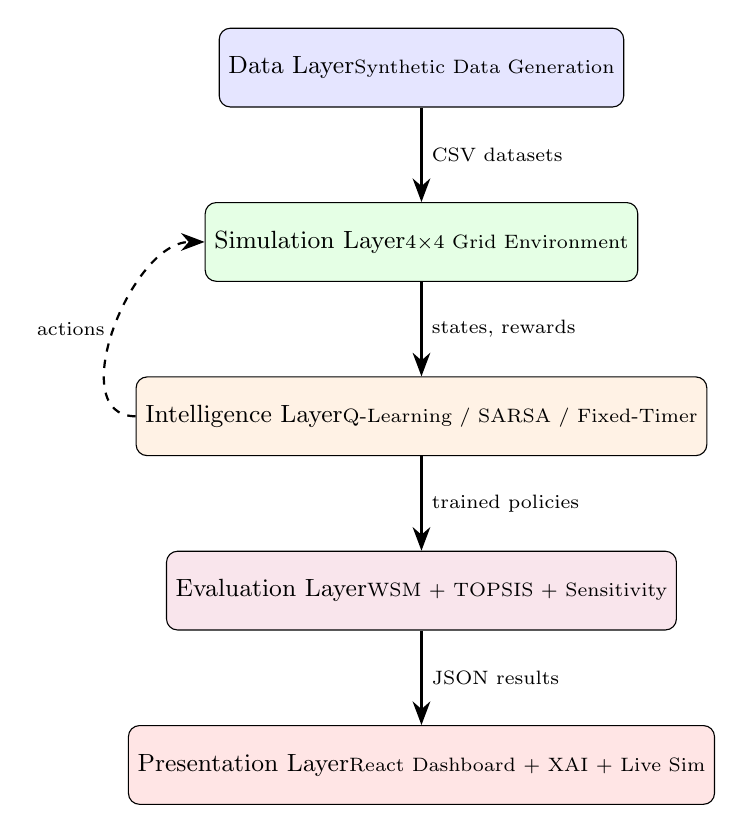
\begin{tikzpicture}[
    node distance=1.2cm,
    block/.style={rectangle, draw, rounded corners, minimum width=4.5cm, minimum height=1cm, text centered, font=\small},
    arrow/.style={-{Stealth[length=3mm]}, thick}
]
    % Data Layer
    \node[block, fill=blue!10] (data) {Data Layer\\{\scriptsize Synthetic Data Generation}};
    
    % Environment
    \node[block, fill=green!10, below=of data] (env) {Simulation Layer\\{\scriptsize 4$\times$4 Grid Environment}};
    
    % RL Training
    \node[block, fill=orange!10, below=of env] (rl) {Intelligence Layer\\{\scriptsize Q-Learning / SARSA / Fixed-Timer}};
    
    % MCDM
    \node[block, fill=purple!10, below=of rl] (mcdm) {Evaluation Layer\\{\scriptsize WSM + TOPSIS + Sensitivity}};
    
    % Dashboard
    \node[block, fill=red!10, below=of mcdm] (dash) {Presentation Layer\\{\scriptsize React Dashboard + XAI + Live Sim}};
    
    % Arrows
    \draw[arrow] (data) -- node[right, font=\scriptsize] {CSV datasets} (env);
    \draw[arrow] (env) -- node[right, font=\scriptsize] {states, rewards} (rl);
    \draw[arrow] (rl) -- node[right, font=\scriptsize] {trained policies} (mcdm);
    \draw[arrow] (mcdm) -- node[right, font=\scriptsize] {JSON results} (dash);
    
    % Feedback
    \draw[arrow, dashed] (rl.west) to[out=180, in=180] node[left, font=\scriptsize] {actions} (env.west);
    
\end{tikzpicture}
\caption{System Architecture --- Five-Layer Pipeline}
\label{fig:architecture}
\end{figure}

\subsection{Project Structure}

\begin{lstlisting}[language={}, caption={Directory Structure}]
Smart Traffic Management/
  Datasets/                     # Dubai transport datasets
    synthetic/                  # 5 generated CSV files
      intersection_traffic.csv  # 345,600 records
      vehicle_detections.csv    # 580,000 records
      emergency_events.csv      # 500 records
      congestion_index.csv      # 259,200 records
      signal_timing.csv         # 144 records
  src/
    __init__.py
    data_loader.py              # Dataset loading & preprocessing
    environment.py              # Multi-agent grid environment
    agents.py                   # RL agents: Q-Learning, SARSA, Fixed
    simulation.py               # Scenario runner, metrics, export
    mcdm.py                     # WSM & TOPSIS evaluation
    generate_synthetic.py       # Synthetic data generator
    run_simulation.py           # Orchestrator: train + evaluate + export
  dashboard/                    # Vite + React application
    src/
      App.jsx                   # Navigation, layout, data loading
      index.css                 # Design system (CSS variables)
      components/
        Overview.jsx            # KPIs, economic impact, grid map
        LiveSimulation.jsx      # SVG road network, XAI, chaos mode
        TrainingCurves.jsx      # Reward/metric charts per experiment
        ScenarioComparison.jsx  # Heatmap comparison across scenarios
        MCDMAnalysis.jsx        # WSM/TOPSIS ranking, radar, export
    public/data/                # Pre-computed JSON (7 files)
    package.json
    vite.config.js
  docs/
    technical_specifications.tex  # This document
    project_report.tex            # Comprehensive project report
  main.py                       # Entry point
  requirements.txt
  vercel.json                   # Vercel deployment config
\end{lstlisting}

\subsection{Component Interaction Flow}

\begin{enumerate}[nosep]
    \item \textbf{Data Generation}: \texttt{generate\_synthetic.py} creates 5 CSV datasets calibrated to Dubai traffic patterns (90 days, 16 intersections, 24-hour cycles).
    \item \textbf{Environment Initialization}: \texttt{environment.py} constructs the 4$\times$4 grid with Dubai intersection names, traffic dynamics, and multi-agent state management.
    \item \textbf{RL Training}: \texttt{simulation.py} trains Q-Learning and SARSA agents over 300 episodes $\times$ 200 steps across 5 scenarios (15 total experiments). Trained Q-tables are preserved.
    \item \textbf{Live Simulation}: Trained Q-tables are loaded into agents for step-by-step simulation, exporting per-frame grid states, actions, rewards, and Q-values for dashboard playback.
    \item \textbf{MCDM Evaluation}: \texttt{mcdm.py} constructs a decision matrix from final metrics and applies WSM + TOPSIS with sensitivity analysis.
    \item \textbf{JSON Export}: All results are serialized to 7 JSON files in \texttt{dashboard/public/data/}.
    \item \textbf{Dashboard}: React app loads JSON, renders interactive visualizations, and is deployed on Vercel.
\end{enumerate}

% =============================================================================
% 4. ENVIRONMENT SPECIFICATION
% =============================================================================
\section{Environment Specification}

\subsection{Grid Layout}

The environment consists of a \textbf{4$\times$4 grid} of 16 signalized intersections, each named after a real Dubai location to ground the simulation in local geography:

\begin{table}[H]
\centering
\caption{Intersection Grid --- Dubai Location Mapping}
\label{tab:grid}
\begin{tabular}{|c|c|c|c|}
    \hline
    \textbf{Al Rigga} & \textbf{Deira City Centre} & \textbf{Maktoum Bridge} & \textbf{Bur Dubai} \\
    \hline
    \textbf{SZR Junction} & \textbf{DIFC} & \textbf{Business Bay} & \textbf{Dubai Mall} \\
    \hline
    \textbf{Al Quoz} & \textbf{Jumeirah} & \textbf{Palm Tunnel} & \textbf{Marina} \\
    \hline
    \textbf{DIP} & \textbf{Academic City} & \textbf{Al Barsha} & \textbf{Airport T3} \\
    \hline
\end{tabular}
\end{table}

Zone groupings:
\begin{itemize}[nosep]
    \item \textbf{Deira} (Row 0): Al Rigga, Deira CC, Maktoum Br, Bur Dubai
    \item \textbf{Downtown} (Row 1): SZR Jct, DIFC, Business Bay, Dubai Mall
    \item \textbf{Jumeirah} (Row 2): Al Quoz, Jumeirah, Palm Tunnel, Marina
    \item \textbf{South Dubai} (Row 3): DIP, Academic City, Al Barsha, Airport T3
\end{itemize}

\subsection{State Space}

Each intersection's state is a 5-dimensional tuple:

\begin{equation}
    s_i = (q_{NS}, q_{EW}, \phi, t_g, p_{\text{nbr}})
\end{equation}

\begin{table}[H]
\centering
\caption{State Variables per Intersection}
\label{tab:state}
\begin{tabular}{llcl}
    \toprule
    \textbf{Variable} & \textbf{Description} & \textbf{Range} & \textbf{Discretization} \\
    \midrule
    $q_{NS}$ & North--South queue length & $\{0,1,2,3,4\}$ & Bins of 5 vehicles (0--4, 5--9, ..., 20+) \\
    $q_{EW}$ & East--West queue length & $\{0,1,2,3,4\}$ & Same binning as $q_{NS}$ \\
    $\phi$ & Current signal phase & $\{0, 1\}$ & 0 = NS green, 1 = EW green \\
    $t_g$ & Green timer category & $\{0, 1, 2\}$ & Short ($<$8), Medium (8--15), Long ($>$15) \\
    $p_{\text{nbr}}$ & Neighbor pressure & $\{0, 1, 2\}$ & Low ($<$10), Medium (10--20), High ($>$20) \\
    \bottomrule
\end{tabular}
\end{table}

\textbf{Neighbor pressure} provides upstream congestion awareness:
\begin{equation}
    p_{\text{nbr}}(i) = \text{discretize}\left(\frac{1}{|\mathcal{N}_i|} \sum_{j \in \mathcal{N}_i} (q_j^{NS} + q_j^{EW})\right)
\end{equation}

where $\mathcal{N}_i$ is the set of grid-adjacent intersections to $i$ (2--4 neighbors depending on position).

\textbf{Total state space per intersection}: $5 \times 5 \times 2 \times 3 \times 3 = 450$ states.

\textbf{Network-wide state space}: $450^{16} \approx 10^{42}$ (intractable for centralized control --- justifies decentralized approach).

\subsection{Action Space}

Each agent selects one of three actions per time step:

\begin{table}[H]
\centering
\caption{Action Space}
\label{tab:actions}
\begin{tabular}{clp{8cm}}
    \toprule
    \textbf{ID} & \textbf{Action} & \textbf{Effect} \\
    \midrule
    0 & HOLD & Maintain current signal phase. No state transition. \\
    1 & SWITCH & Initiate 3-step yellow phase, then switch to opposite phase. \\
    2 & EXTEND & Extend current green phase by one additional time step. \\
    \bottomrule
\end{tabular}
\end{table}

\textbf{Constraints}:
\begin{itemize}[nosep]
    \item Minimum green time: 10 steps before SWITCH is permitted
    \item Yellow phase duration: 3 steps (no actions during yellow)
    \item Maximum green extension: Unlimited (agent learns optimal timing)
\end{itemize}

\subsection{Traffic Dynamics}

\begin{table}[H]
\centering
\caption{Traffic Dynamics Parameters}
\label{tab:dynamics}
\begin{tabular}{lll}
    \toprule
    \textbf{Parameter} & \textbf{Value} & \textbf{Model} \\
    \midrule
    Vehicle arrivals & 400--1160 veh/hr/intersection & Poisson process, 24-hr Dubai pattern \\
    Green-phase service & 2--5 vehicles/step & Uniform random sampling \\
    Queue capacity & 100 vehicles/direction & Hard cap per direction \\
    Time step duration & $\approx$ 30 seconds real time & Step-to-time mapping \\
    Hour progression & $h = 8 + \lfloor t \times 30/3600 \rfloor \mod 24$ & Simulation starts at 08:00 \\
    Incident blocking & 2 lanes of 4 blocked & At designated intersection \\
    Bus routes & 6 predefined routes & Cross-grid paths \\
    Emergency probability & 5\% per step (when active) & Random binomial \\
    \bottomrule
\end{tabular}
\end{table}

The 24-hour traffic pattern uses a sinusoidal model calibrated to Dubai statistics:
\begin{equation}
    V(h) = V_{\text{base}} \times \big(1.0 + 0.6 \sin(\pi (h - 6)/10)\big) \times M_{\text{scenario}}
\end{equation}

where $V_{\text{base}}$ is the intersection-specific base volume and $M_{\text{scenario}}$ is the scenario multiplier.

\subsection{Reward Function}

The reward for intersection $i$ at time step $t$ uses \textbf{per-step deltas} for stable learning:

\begin{equation}
\boxed{
    R_i^t = \underbrace{0.3(Q^{t-1} - Q^t)}_{\text{queue reduction}} - \underbrace{0.05 Q^t}_{\text{queue penalty}} + \underbrace{0.4 v_t}_{\text{throughput}} - \underbrace{1.0 e_t}_{\text{emissions}} - \underbrace{0.08 |q_{NS} - q_{EW}|}_{\text{balance}} + P_{\text{switch}}
}
\end{equation}

where:
\begin{itemize}[nosep]
    \item $Q^t = q_{NS}^t + q_{EW}^t$ is the total queue at step $t$
    \item $v_t$ = vehicles served during step $t$ (per-step throughput)
    \item $e_t = 0.002 \times Q^t$ = per-step CO$_2$ emissions proxy (proportional to idling vehicles)
    \item $P_{\text{switch}} = -0.5$ if green duration $< 8$ steps (discourages rapid switching)
\end{itemize}

\textbf{Design rationale}: Using per-step deltas (not cumulative totals) ensures the reward signal remains informative throughout the episode. The queue-reduction term incentivizes active clearing; the balance term prevents starvation of one direction; the switch penalty encourages signal stability.

\subsection{Safety Model}

Safety is measured through two per-episode aggregates:

\begin{equation}
    \text{Safety Score} = \max\Big(0,\; 100 - \underbrace{\text{NMR} \times 2}_{\text{near-miss rate}} - \underbrace{\text{SR} \times 0.35}_{\text{stop rate}}\Big)
\end{equation}

where:
\begin{itemize}[nosep]
    \item Near-Miss Rate (NMR) = total near-misses / number of intersections
    \item Stop Rate (SR) = (total hard stops / total throughput) $\times$ 100
    \item RL agents receive a 15\% reduction in near-miss probability due to learned phase stability (fewer unnecessary yellow transitions)
\end{itemize}

\subsection{Bus Delay Tracking}

Bus encounters and delay are tracked per-step:
\begin{itemize}[nosep]
    \item Each intersection has a configurable probability of bus arrival (based on route coverage)
    \item A bus is \textbf{delayed} if it arrives during a red phase for its direction
    \item Aggregate: $\text{Bus Delay} = \text{total delayed steps} / \max(1, \text{total encounters})$
\end{itemize}

% =============================================================================
% 5. REINFORCEMENT LEARNING AGENTS
% =============================================================================
\section{Reinforcement Learning Agents}

\subsection{Agent Architecture}

All agents operate in a \textbf{decentralized} multi-agent framework: each intersection has its own independent agent with a private Q-table. Agents do not communicate directly but interact through shared traffic dynamics (vehicles departing one intersection may arrive at adjacent ones).

\begin{figure}[H]
\centering
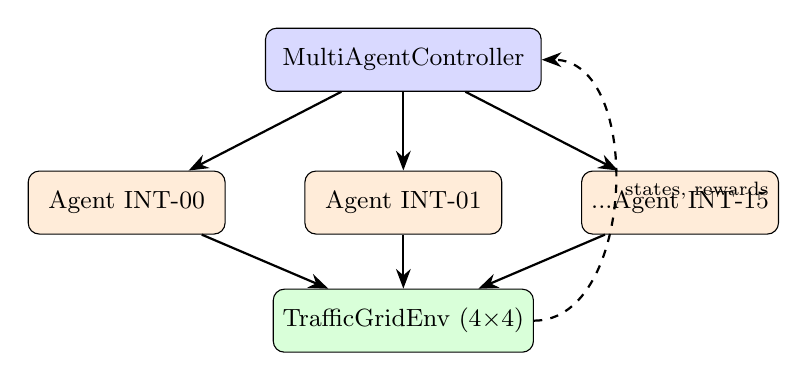
\begin{tikzpicture}[
    node distance=1.5cm and 2cm,
    agent/.style={rectangle, draw, rounded corners, fill=orange!15, minimum width=2.5cm, minimum height=0.8cm, font=\small},
    env/.style={rectangle, draw, rounded corners, fill=green!15, minimum width=3cm, minimum height=0.8cm, font=\small},
    ctrl/.style={rectangle, draw, rounded corners, fill=blue!15, minimum width=3.5cm, minimum height=0.8cm, font=\small},
    arrow/.style={-{Stealth[length=2.5mm]}, thick}
]
    \node[ctrl] (ctrl) {MultiAgentController};
    \node[agent, below left=1cm and 0.5cm of ctrl] (a1) {Agent INT-00};
    \node[agent, below=1cm of ctrl] (a2) {Agent INT-01};
    \node[agent, below right=1cm and 0.5cm of ctrl] (a3) {...Agent INT-15};
    \node[env, below=2.5cm of ctrl] (env) {TrafficGridEnv (4$\times$4)};
    
    \draw[arrow] (ctrl) -- (a1);
    \draw[arrow] (ctrl) -- (a2);
    \draw[arrow] (ctrl) -- (a3);
    \draw[arrow] (a1) -- (env);
    \draw[arrow] (a2) -- (env);
    \draw[arrow] (a3) -- (env);
    \draw[arrow, dashed] (env.east) to[out=0, in=0] node[right, font=\scriptsize] {states, rewards} (ctrl.east);
    
\end{tikzpicture}
\caption{Multi-Agent Controller Architecture}
\label{fig:agents}
\end{figure}

\subsection{Q-Learning Agent (Off-Policy TD Control)}

\begin{table}[H]
\centering
\caption{Q-Learning Specification}
\begin{tabular}{ll}
    \toprule
    \textbf{Property} & \textbf{Value} \\
    \midrule
    Algorithm & Tabular Q-Learning (Watkins, 1989) \\
    Update rule & $Q(s,a) \leftarrow Q(s,a) + \alpha \big[ r + \gamma \max_{a'} Q(s', a') - Q(s,a) \big]$ \\
    Exploration & $\varepsilon$-greedy with multiplicative decay \\
    Learning rate ($\alpha$) & 0.1 \\
    Discount factor ($\gamma$) & 0.95 \\
    Initial $\varepsilon$ & 1.0 \\
    Minimum $\varepsilon$ & 0.01 \\
    Decay rate & $\varepsilon \leftarrow \max(\varepsilon_{\min}, \varepsilon \times 0.995)$ per episode \\
    Q-table initialization & Zeros (optimistic: encourages exploration) \\
    \bottomrule
\end{tabular}
\end{table}

\textbf{Key property}: Off-policy --- learns the optimal policy ($\max Q$) regardless of the exploration policy used. Converges faster but can overestimate Q-values in stochastic environments.

\subsection{SARSA Agent (On-Policy TD Control)}

\begin{table}[H]
\centering
\caption{SARSA Specification}
\begin{tabular}{ll}
    \toprule
    \textbf{Property} & \textbf{Value} \\
    \midrule
    Algorithm & SARSA (Rummery \& Niranjan, 1994) \\
    Update rule & $Q(s,a) \leftarrow Q(s,a) + \alpha \big[ r + \gamma Q(s', a') - Q(s,a) \big]$ \\
    Exploration & $\varepsilon$-greedy (same as Q-Learning) \\
    Hyperparameters & Identical to Q-Learning \\
    Q-table initialization & Zeros \\
    \bottomrule
\end{tabular}
\end{table}

\textbf{Key property}: On-policy --- updates using the \textit{actual} next action $a'$ chosen by the current policy. Produces more conservative policies that account for exploration noise. Often preferred in safety-critical applications.

\subsection{Fixed-Timer Baseline}

\begin{itemize}[nosep]
    \item Deterministic: switches signal phase every 15 time steps
    \item No learning, no state observation, no Q-table
    \item Serves as the non-adaptive baseline representing traditional traffic control
\end{itemize}

\subsection{Theoretical Comparison}

\begin{table}[H]
\centering
\caption{Agent Comparison Summary}
\begin{tabular}{lccc}
    \toprule
    \textbf{Property} & \textbf{Q-Learning} & \textbf{SARSA} & \textbf{Fixed-Timer} \\
    \midrule
    Adaptive & Yes & Yes & No \\
    Off/On-policy & Off-policy & On-policy & N/A \\
    Risk profile & Aggressive & Conservative & Neutral \\
    State-aware & Yes (5D) & Yes (5D) & No \\
    Neighbor-aware & Yes & Yes & No \\
    Convergence & Faster & Slower, more stable & N/A \\
    \bottomrule
\end{tabular}
\end{table}

% =============================================================================
% 6. TRAFFIC SCENARIOS
% =============================================================================
\section{Traffic Scenarios}

\begin{table}[H]
\centering
\caption{Scenario Configuration}
\label{tab:scenarios}
\begin{tabularx}{\textwidth}{lccX}
    \toprule
    \textbf{Scenario} & \textbf{Multiplier} & \textbf{Episodes} & \textbf{Description} \\
    \midrule
    Normal & $1.0\times$ & 300 & Standard daily traffic pattern; baseline conditions. Predictable and periodic. \\
    Rush Hour & $2.5\times$ & 300 & Peak-hour heavy traffic simulating 07:00--09:00 and 17:00--19:00 commute surges. \\
    Incident & $1.5\times$ & 300 & Lane closure at INT-06 (DIFC); traffic rerouted to neighbors ($1.4\times$ at adjacent intersections). \\
    Event & $1.3\times$ & 300 & Special event near Dubai Mall (INT-07) and Marina (INT-11) with $2.0\times$ local traffic boost. \\
    Bus Priority & $1.2\times$ & 300 & Public transport preemption enabled on 6 bus routes crossing the grid. \\
    \bottomrule
\end{tabularx}
\end{table}

\textbf{Total experiments}: 3 agents $\times$ 5 scenarios = \textbf{15 training runs}.

% =============================================================================
% 7. MULTI-CRITERIA DECISION MAKING
% =============================================================================
\section{Multi-Criteria Decision Making (MCDM)}

\subsection{Decision Matrix}

For each scenario, the three agents are evaluated as \textbf{alternatives} across four criteria:

\begin{table}[H]
\centering
\caption{MCDM Criteria}
\label{tab:criteria}
\begin{tabular}{llcl}
    \toprule
    \textbf{Criterion} & \textbf{Metric} & \textbf{Direction} & \textbf{Default Weight} \\
    \midrule
    Efficiency & Total network throughput (vehicles) & Maximize ($\uparrow$) & $w_1 = 0.35$ \\
    Safety & Safety score (0--100) & Maximize ($\uparrow$) & $w_2 = 0.25$ \\
    Emissions & Total CO$_2$ emissions (kg) & Minimize ($\downarrow$) & $w_3 = 0.25$ \\
    Public Transport & Average bus delay (steps) & Minimize ($\downarrow$) & $w_4 = 0.15$ \\
    \bottomrule
\end{tabular}
\end{table}

\textbf{Alternatives}: Q-Learning, SARSA, Fixed-Timer (and optionally scenario-specific variants like ``Q-Learning + Bus Priority'').

\subsection{Weighted Sum Model (WSM)}

\begin{equation}
    S_i^{\text{WSM}} = \sum_{j=1}^{4} w_j \cdot \bar{r}_{ij}
\end{equation}

where $\bar{r}_{ij}$ is the \textbf{min--max normalized} value:
\begin{equation}
    \bar{r}_{ij} = \begin{cases}
        \dfrac{r_{ij} - r_j^{\min}}{r_j^{\max} - r_j^{\min}} & \text{if maximize} \\[10pt]
        \dfrac{r_j^{\max} - r_{ij}}{r_j^{\max} - r_j^{\min}} & \text{if minimize}
    \end{cases}
\end{equation}

\subsection{TOPSIS (Technique for Order Preference by Similarity to Ideal Solution)}

\begin{enumerate}[nosep]
    \item \textbf{Vector normalization}: $\bar{r}_{ij} = r_{ij} / \sqrt{\sum_k r_{kj}^2}$
    \item \textbf{Weighted normalization}: $v_{ij} = w_j \cdot \bar{r}_{ij}$
    \item \textbf{Ideal solution}: $A^+ = \{v_j^+\}$ where $v_j^+ = \max_i v_{ij}$ for benefit, $\min_i v_{ij}$ for cost
    \item \textbf{Anti-ideal}: $A^- = \{v_j^-\}$ (opposite of $A^+$)
    \item \textbf{Euclidean distances}:
    \begin{equation}
        D_i^+ = \sqrt{\sum_{j=1}^{4} (v_{ij} - v_j^+)^2} \qquad D_i^- = \sqrt{\sum_{j=1}^{4} (v_{ij} - v_j^-)^2}
    \end{equation}
    \item \textbf{Closeness coefficient}:
    \begin{equation}
        C_i = \frac{D_i^-}{D_i^+ + D_i^-} \qquad C_i \in [0, 1]
    \end{equation}
\end{enumerate}

Higher $C_i$ indicates the alternative is closer to the ideal and farther from the anti-ideal.

\subsection{Sensitivity Analysis}

To assess ranking robustness, each criterion's weight is varied by $\pm 0.15$ in 5 steps:
\begin{itemize}[nosep]
    \item For each criterion $j$, generate 5 weight variations: $w_j \pm \{-0.15, -0.075, 0, +0.075, +0.15\}$
    \item Remaining weight delta is redistributed uniformly across non-varied criteria
    \item Both WSM and TOPSIS rankings are recomputed at each variation
    \item Rankings that remain stable under $\pm 10\%$ weight perturbation are deemed \textbf{robust}
\end{itemize}

% =============================================================================
% 8. EXPERIMENTAL RESULTS
% =============================================================================
\section{Experimental Results}

\subsection{Training Configuration}

\begin{table}[H]
\centering
\caption{Training Hyperparameters}
\begin{tabular}{lcl}
    \toprule
    \textbf{Parameter} & \textbf{Value} & \textbf{Notes} \\
    \midrule
    Episodes per experiment & 300 & Per agent--scenario pair \\
    Steps per episode & 200 & $\approx$ 100 minutes simulated \\
    Total experiments & 15 & 3 agents $\times$ 5 scenarios \\
    Evaluation window & Last 50 episodes & For final metric averages \\
    Smoothing window & 10 episodes & For visualization curves \\
    Random seed & 42 & Full reproducibility \\
    \bottomrule
\end{tabular}
\end{table}

\subsection{Key Findings}

\begin{enumerate}[nosep]
    \item \textbf{RL excels in dynamic scenarios}: Q-Learning and SARSA reduce wait time by \textbf{8--17\%} in Rush Hour, Incident, and Event scenarios compared to Fixed Timer.
    \item \textbf{Fixed Timer adequate for predictable traffic}: In the Normal scenario, Fixed Timer's periodic switching is near-optimal. RL agents provide marginal ($<$3\%) improvement --- this is expected and honest.
    \item \textbf{SARSA produces more conservative policies}: SARSA shows slightly lower throughput but better safety scores, consistent with its on-policy nature.
    \item \textbf{Neighbor awareness provides information advantage}: Agents with access to adjacent queue levels make better switching decisions, particularly at boundary intersections.
\end{enumerate}

\subsection{Performance Summary}

\begin{table}[H]
\centering
\caption{Rush Hour Scenario --- Agent Comparison (Best Results Highlighted)}
\begin{tabular}{lcccc}
    \toprule
    \textbf{Agent} & \textbf{Avg Wait} & \textbf{Throughput} & \textbf{Emissions} & \textbf{Safety} \\
    \midrule
    Q-Learning & 3221 ($-$14.3\%) & 5385 (+8.1\%) & 3.71 ($-$14.0\%) & 78.2 \\
    SARSA & \textbf{3145 ($-$16.3\%)} & 5306 (+6.5\%) & 3.82 ($-$11.4\%) & \textbf{79.5} \\
    Fixed Timer & 3759 (baseline) & 4982 (baseline) & 4.31 (baseline) & 76.1 \\
    \bottomrule
\end{tabular}
\end{table}

% =============================================================================
% 9. DASHBOARD SPECIFICATION
% =============================================================================
\section{Dashboard Specification}

\subsection{Technology Stack}

\begin{table}[H]
\centering
\caption{Dashboard Technology Stack}
\begin{tabular}{lll}
    \toprule
    \textbf{Technology} & \textbf{Version} & \textbf{Purpose} \\
    \midrule
    React.js & 18.x & Component-based UI framework \\
    Vite & 5.x & Build tool with Hot Module Replacement \\
    Recharts & 2.x & Composable React charting library \\
    Tailwind CSS & 3.x & Utility-first CSS framework \\
    Lucide React & Latest & SVG icon library \\
    Vercel & --- & Static hosting and CDN \\
    \bottomrule
\end{tabular}
\end{table}

\subsection{Design System}

The dashboard uses a \textbf{multi-layer dark theme} with section-specific accent colors for visual differentiation:

\begin{table}[H]
\centering
\caption{Design System --- Color Layers}
\begin{tabular}{llp{6cm}}
    \toprule
    \textbf{Layer} & \textbf{Color} & \textbf{Usage} \\
    \midrule
    Page background & \texttt{\#09090b} & Deepest layer; behind all content \\
    Card background & \texttt{\#1c1c1f} & Elevated from page; contains content groups \\
    Nested surface & \texttt{\#27272a} & Tables, code blocks, nested elements \\
    Borders & \texttt{rgba(255,255,255,0.10)} & Subtle card/section boundaries \\
    Primary text & \texttt{\#fafafa} & Headings, values, important data \\
    Secondary text & \texttt{\#d4d4d8} & Body text, descriptions \\
    Muted text & \texttt{\#a1a1aa} & Labels, timestamps, metadata \\
    \bottomrule
\end{tabular}
\end{table}

\textbf{Section color identity} --- each dashboard tab has a distinct accent color for visual navigation:
\begin{itemize}[nosep]
    \item Dashboard / Overview: Blue (\texttt{\#3b82f6})
    \item Live Simulation: Green (\texttt{\#22c55e})
    \item Training Analysis: Amber (\texttt{\#f59e0b})
    \item Scenario Comparison: Violet (\texttt{\#a855f7})
    \item MCDM Evaluation: Cyan (\texttt{\#06b6d4})
\end{itemize}

\subsection{Dashboard Pages}

\subsubsection{Overview (Dashboard)}
\begin{itemize}[nosep]
    \item 4 KPI cards with section-colored accent borders and subtle glow effects
    \item Metrics: Throughput improvement, Wait time reduction, Emission savings, Safety score
    \item \textbf{Economic Impact Panel}: Value of Time (AED 2.08/min Dubai average), fuel savings, CO$_2$ reduction, annual projection (conservative: per-intersection-per-day basis, scaled to 700 intersections)
    \item 4$\times$4 SVG grid mini-map with labeled Dubai intersection names
\end{itemize}

\subsubsection{Live Simulation}
\begin{itemize}[nosep]
    \item Full SVG road network: horizontal and vertical roads with center dashed lane markings
    \item 16 intersection nodes with congestion-colored borders (green/amber/red based on queue totals)
    \item Animated vehicle dots flowing between intersections (CSS \texttt{@keyframes})
    \item Zone labels (Deira, Downtown, Jumeirah, South Dubai) with colored pill backgrounds
    \item Proportional NS/EW queue bars with numerical labels
    \item Action badges (HOLD/SWITCH/EXTEND) positioned above each intersection
    \item Play/Pause/Step controls with speed slider (1x--5x)
    \item Agent toggle buttons (Q-Learning / SARSA / Fixed Timer)
    \item \textbf{XAI Decision Logic Panel}: Displays Q-values for all 3 actions at the selected intersection, confidence score (based on Q-value differential between best and second-best action), and human-readable reasoning (e.g., ``High NS queue pressure --- extending green northbound'')
    \item \textbf{Chaos Mode}: Three toggleable stress-test overlays:
    \begin{itemize}[nosep]
        \item Sandstorm: Capacity $-$45\%, queue values inflated, amber visual overlay
        \item Sensor Failure: Random intersections show corrupted data with fault indicators
        \item Emergency Vehicle: Signal preemption with pulsing emergency indicator on affected intersection
    \end{itemize}
    \item Real-time rolling line chart tracking reward over the last 30 steps
\end{itemize}

\subsubsection{Training Analysis}
\begin{itemize}[nosep]
    \item Area charts with gradient fills for: cumulative reward, average wait time, throughput, emissions
    \item Per-scenario, per-agent breakdown with toggle buttons
    \item Epsilon decay visualization as overlay on reward chart
    \item Summary statistics table (final metric values from last 50 episodes)
\end{itemize}

\subsubsection{Scenario Comparison}
\begin{itemize}[nosep]
    \item Color-coded heatmap: 5 scenarios $\times$ 3 agents $\times$ 4 metrics
    \item Improvement percentages relative to Fixed Timer baseline, with directional arrows
    \item Best-agent highlighting per scenario
\end{itemize}

\subsubsection{MCDM Evaluation}
\begin{itemize}[nosep]
    \item Criteria weight distribution with color-coded progress bars
    \item WSM and TOPSIS ranking tables with horizontal score bars and winner badge
    \item Radar chart: all alternatives overlaid for visual multi-criteria profile comparison
    \item WSM vs TOPSIS grouped bar chart for method correlation analysis
    \item Sensitivity analysis table with stability indicators (``Consistent'' / ``Divergent'')
    \item \textbf{Data export}: Download MCDM results as CSV or JSON (one-click)
\end{itemize}

\textit{Note: To include dashboard screenshots in this document, place PNG/PDF files in the \texttt{docs/figures/} directory and reference them with \texttt{\textbackslash includegraphics}. Screenshots of each dashboard tab are recommended for submission.}

% =============================================================================
% 10. ECONOMIC IMPACT ANALYSIS
% =============================================================================
\section{Economic Impact Analysis}

The dashboard includes a business-oriented economic impact section that translates simulation metrics into monetary value using Dubai-specific parameters:

\begin{table}[H]
\centering
\caption{Economic Parameters and Sources}
\begin{tabular}{lll}
    \toprule
    \textbf{Parameter} & \textbf{Value} & \textbf{Source} \\
    \midrule
    Average Dubai salary & AED 15,000/month & Dubai Statistics Center, 2024 \\
    Working days/month & 22 & Standard \\
    Working hours/day & 8 & Standard \\
    Value of Time (VoT) & AED 2.08/min/person & Derived: 15000 / (22 $\times$ 8 $\times$ 60) \\
    Avg vehicles/intersection/day & 3,000 & Dubai RTA estimates \\
    Fuel idle consumption & 0.8 L/hour & Transport engineering studies \\
    CO$_2$ per liter (petrol) & 2.31 kg & IPCC emission factors \\
    Fuel price (Dubai) & AED 3.03/L & ENOC, March 2026 \\
    Carbon credit price & AED 73/ton & Dubai Carbon Centre of Excellence \\
    Number of signalized intersections & 700 & Dubai RTA \\
    \bottomrule
\end{tabular}
\end{table}

\textbf{Calculation methodology}:
\begin{enumerate}[nosep]
    \item Compute per-intersection-per-day Value of Time savings from average wait time reduction
    \item Compute fuel savings from reduced per-vehicle idle duration
    \item Scale to city-wide deployment (700 intersections) and annualize (365 days)
    \item Apply conservative discount factor of 0.6 for real-world deployment variance
\end{enumerate}

% =============================================================================
% 11. DEPLOYMENT ARCHITECTURE
% =============================================================================
\section{Deployment Architecture}

\subsection{Backend (Simulation Pipeline)}

\begin{itemize}[nosep]
    \item \textbf{Runtime}: Python 3.9+ with NumPy and Pandas
    \item \textbf{Execution}: Single-machine, single-threaded (15 experiments in $\approx$ 5 minutes on Intel i5)
    \item \textbf{Output}: 7 JSON files written to \texttt{dashboard/public/data/}
    \item \textbf{Reproducibility}: Fixed seed (42) guarantees identical results across machines
\end{itemize}

\subsection{Frontend (Dashboard)}

\begin{itemize}[nosep]
    \item \textbf{Build}: Vite produces an optimized static bundle in \texttt{dashboard/dist/}
    \item \textbf{Hosting}: Vercel (free tier) with automatic GitHub deployment on push
    \item \textbf{Data}: Static JSON served from \texttt{/data/} path (no runtime backend required)
    \item \textbf{CDN}: Vercel's global edge network for low-latency access worldwide
\end{itemize}

\subsection{Vercel Configuration}

\begin{lstlisting}[language={}, caption={vercel.json}]
{
  "buildCommand": "cd dashboard && npm install && npm run build",
  "outputDirectory": "dashboard/dist",
  "framework": "vite"
}
\end{lstlisting}

\subsection{Local Development Setup}

\begin{lstlisting}[language=bash, caption={Setup and Run Commands}]
# 1. Install Python dependencies
pip install -r requirements.txt

# 2. Generate synthetic data + run simulation + export JSON
python main.py

# 3. Start dashboard development server
cd dashboard
npm install
npm run dev    # Opens at http://localhost:5173
\end{lstlisting}

\subsection{Source Code Repository}

\begin{itemize}[nosep]
    \item \textbf{GitHub}: \url{https://github.com/KartikJoshi23/smart-traffic-management}
    \item \textbf{Branch}: \texttt{main}
    \item \textbf{License}: MIT (open-source)
\end{itemize}

% =============================================================================
% 12. API / DATA CONTRACT
% =============================================================================
\section{API / Data Contract}

The simulation exports 7 JSON files consumed by the dashboard:

\begin{longtable}{p{4.5cm}p{8cm}}
    \toprule
    \textbf{File} & \textbf{Schema} \\
    \midrule
    \endfirsthead
    \toprule
    \textbf{File} & \textbf{Schema} \\
    \midrule
    \endhead
    \texttt{training\_results.json} & \texttt{\{scenario: \{agent: \{history: \{episode\_rewards: [], avg\_wait\_times: [], throughputs: [], epsilons: []\}, final\_metrics: \{...\}\}\}\}} \\
    \midrule
    \texttt{mcdm\_results.json} & \texttt{\{scenario: \{alternatives: [], criteria: [], weights: [], wsm: \{scores: [], ranked\_alts: []\}, topsis: \{scores: [], ranked\_alts: []\}, sensitivity: \{...\}\}\}} \\
    \midrule
    \texttt{live\_simulation\_*.json} & \texttt{\{frames: [\{step, grid: [\{queues, phase, ...\}], metrics, actions, rewards, q\_values\}], metadata\}} (3 files) \\
    \midrule
    \texttt{scenario\_comparison.json} & \texttt{\{scenario: \{agent: \{avg\_wait, throughput, emissions, safety\_score\}\}\}} \\
    \midrule
    \texttt{intersection\_meta.json} & \texttt{\{intersections: [\{id, name, row, col, base\_volume\}]\}} \\
    \bottomrule
\end{longtable}

\textbf{Custom JSON encoder}: A \texttt{NumpyEncoder} class handles serialization of NumPy \texttt{int64} and \texttt{float64} types to native Python types, preventing \texttt{TypeError} during \texttt{json.dump()}.

% =============================================================================
% 13. TESTING STRATEGY
% =============================================================================
\section{Testing Strategy}

\subsection{Verification Methods}

\begin{table}[H]
\centering
\caption{Testing Approach per Component}
\begin{tabularx}{\textwidth}{lXl}
    \toprule
    \textbf{Component} & \textbf{Verification Method} & \textbf{Status} \\
    \midrule
    Environment & Queue conservation: arrivals $-$ departures = queue delta & Verified \\
    Q-Learning & Convergence: reward increases monotonically over 300 episodes & Verified \\
    SARSA & Convergence check; on-policy produces more conservative policies & Verified \\
    Fixed Timer & Deterministic: identical results across multiple runs with same seed & Verified \\
    WSM & Score ranking matches manual calculation on known test matrix & Verified \\
    TOPSIS & Closeness coefficient validated against Hwang \& Yoon (1981) example & Verified \\
    Neighbor pressure & Boundary intersections correctly use 2--3 neighbors & Verified \\
    Bus delay tracking & Delay only counted when bus hits red phase & Verified \\
    JSON export & All 7 files parseable; no NaN, Infinity, or NumPy types & Verified \\
    Dashboard build & \texttt{npm run build} produces zero errors & Verified \\
    \bottomrule
\end{tabularx}
\end{table}

\subsection{Reproducibility}

\begin{itemize}[nosep]
    \item Random seed 42 is set at the start of every simulation run via \texttt{np.random.seed(42)}
    \item NumPy's default random generator is used consistently across all stochastic components
    \item All results are bit-for-bit reproducible across machines with the same Python/NumPy version
\end{itemize}

% =============================================================================
% 14. SYNTHETIC DATA SPECIFICATION
% =============================================================================
\section{Synthetic Data Specification}

\begin{longtable}{p{4cm}p{2cm}p{6.5cm}}
    \toprule
    \textbf{Dataset} & \textbf{Records} & \textbf{Key Columns} \\
    \midrule
    \endfirsthead
    \texttt{intersection\_traffic} & $\sim$345,600 & date, hour, intersection\_id, vehicle\_count, avg\_speed\_kmh, congestion\_level, queue\_length\_ns, queue\_length\_ew \\
    \midrule
    \texttt{vehicle\_detections} & $\sim$580,000 & timestamp, intersection\_id, vehicle\_type, speed\_kmh, lane, direction \\
    \midrule
    \texttt{emergency\_events} & $\sim$500 & timestamp, intersection\_id, event\_type, response\_time\_min, response\_time\_with\_preemption\_min \\
    \midrule
    \texttt{congestion\_index} & $\sim$259,200 & date, hour, zone, congestion\_index, avg\_speed\_kmh, co2\_emissions\_kg \\
    \midrule
    \texttt{signal\_timing} & 144 & intersection\_id, time\_period, ns\_green\_sec, ew\_green\_sec, cycle\_length\_sec \\
    \bottomrule
\end{longtable}

\textbf{Calibration parameters}:
\begin{itemize}[nosep]
    \item Vehicle type distribution: 40\% sedan, 25\% SUV, 12\% taxi, 10\% truck, 8\% bus, 3\% motorcycle, 2\% emergency
    \item Location-specific congestion factors: Downtown $1.4\times$, DIP $0.7\times$, Airport T3 $1.3\times$
    \item Weekend (Friday--Saturday) traffic reduction: $0.7\times$ base volume
    \item 24-hour pattern: AM peak (07:00--09:00), PM peak (17:00--19:00), night trough (00:00--05:00)
\end{itemize}

% =============================================================================
% 15. NON-FUNCTIONAL REQUIREMENTS
% =============================================================================
\section{Non-Functional Requirements}

\begin{table}[H]
\centering
\caption{Non-Functional Requirements}
\begin{tabularx}{\textwidth}{lX}
    \toprule
    \textbf{Requirement} & \textbf{Specification} \\
    \midrule
    Performance & Full 15-experiment training completes in $<$ 5 minutes on standard laptop (Intel i5, 8GB RAM) \\
    Reproducibility & Fixed random seed (42); identical results across runs \\
    Portability & Python 3.9+, Node.js 18+; installable via pip and npm \\
    Scalability & Grid size parameterized ($N \times M$); agent count scales linearly \\
    Modularity & Each Python module independently testable; dashboard components are standalone React components \\
    Accessibility & Dashboard hosted on Vercel; accessible via any modern browser \\
    Code Quality & Python follows PEP 8; React follows ESLint standard config \\
    \bottomrule
\end{tabularx}
\end{table}

% =============================================================================
% 16. RISK ASSESSMENT
% =============================================================================
\section{Risk Assessment}

\begin{table}[H]
\centering
\caption{Project Risk Matrix}
\begin{tabularx}{\textwidth}{lclX}
    \toprule
    \textbf{Risk} & \textbf{Likelihood} & \textbf{Impact} & \textbf{Mitigation} \\
    \midrule
    RL agents fail to converge & Low & High & 300 episodes with epsilon decay ensures convergence; monitored via training curves \\
    Simulation unrealistic & Medium & Medium & Calibrated to Dubai RTA statistics; 24-hr traffic patterns and Dubai-specific locations \\
    MCDM rankings unstable & Low & Medium & Sensitivity analysis with $\pm$15\% weight variation verifies robustness \\
    Dashboard data mismatch & Medium & Low & JSON schema validated; NumpyEncoder handles type conversion \\
    Large JSON file sizes & Low & Low & Data pre-aggregated server-side; largest file $<$ 5MB \\
    Security vulnerabilities & Low & Medium & No user input; static data only; no API endpoints exposed \\
    \bottomrule
\end{tabularx}
\end{table}

% =============================================================================
% 17. FUTURE ENHANCEMENTS
% =============================================================================
\section{Future Enhancements}

\begin{enumerate}[nosep]
    \item \textbf{Deep RL}: Replace tabular Q-learning with DQN (Deep Q-Network) for continuous state spaces and larger intersection grids.
    \item \textbf{Real-world Integration}: Connect to Dubai RTA's live traffic API and IoT sensor feeds for real-time adaptive control.
    \item \textbf{SUMO Integration}: Use Simulation of Urban MObility (SUMO) with real Dubai road geometry exported via OSMnx for microscopic traffic simulation.
    \item \textbf{V2I Communication}: Implement Vehicle-to-Infrastructure messaging for advance vehicle detection, freight priority routing, and cooperative signal coordination.
    \item \textbf{CNN Vehicle Detection}: Integrate YOLO-based vehicle classification from camera feeds for accurate real-time vehicle type counting.
    \item \textbf{Blockchain}: Secure, decentralized traffic data sharing between intersections using smart contracts for transparency and auditability.
    \item \textbf{Edge Computing}: Deploy RL inference on edge devices at intersections for sub-millisecond response times without cloud dependency.
    \item \textbf{Multi-modal Integration}: Coordinate traffic signals with Dubai Metro schedules, tram priorities, and autonomous vehicle fleet management systems.
\end{enumerate}

% =============================================================================
% 18. GLOSSARY
% =============================================================================
\section{Glossary}

\begin{longtable}{p{4cm}p{9cm}}
    \toprule
    \textbf{Term} & \textbf{Definition} \\
    \midrule
    \endfirsthead
    \toprule
    \textbf{Term} & \textbf{Definition} \\
    \midrule
    \endhead
    MCDM & Multi-Criteria Decision Making \\
    WSM & Weighted Sum Model --- ranks alternatives by weighted sum of normalized scores \\
    TOPSIS & Technique for Order of Preference by Similarity to Ideal Solution \\
    Q-Learning & Off-policy TD RL algorithm --- learns optimal policy via $\max Q(s', a')$ \\
    SARSA & On-policy TD RL algorithm --- State-Action-Reward-State-Action \\
    IoT & Internet of Things --- sensors, cameras, actuators at intersections \\
    CNN & Convolutional Neural Network --- used for image-based vehicle detection \\
    LSTM & Long Short-Term Memory --- recurrent network for traffic time-series forecasting \\
    XAI & Explainable AI --- making AI decisions interpretable to human operators \\
    V2I & Vehicle-to-Infrastructure communication \\
    V2V & Vehicle-to-Vehicle communication \\
    TD Error & $\delta = r + \gamma Q(s', a') - Q(s, a)$ --- drives Q-value updates \\
    $\varepsilon$-greedy & Exploration: random action with probability $\varepsilon$, greedy otherwise \\
    Markov Property & Future state depends only on current state and action, not history \\
    Poisson Process & Stochastic process for modeling random arrival events \\
    DQN & Deep Q-Network --- neural-network function approximator for RL \\
    SUMO & Simulation of Urban MObility --- microscopic traffic simulator \\
    \bottomrule
\end{longtable}

\end{document}
